% CREATED BY DAVID FRISK, 2016
% MODIFIED BY JAKOB JARMAR, 2016
% A few changes by Birgit Grohe, 2017 and 2018
% Adjustments with the help of Gustav Örtenberg 2019

% IMPORT SETTINGS
\documentclass[12pt,a4paper,twoside,openright]{report}
% CREATED BY DAVID FRISK, 2016

% BASIC SETTINGS
\usepackage{moreverb}								% List settings
\usepackage{textcomp}								% Fonts, symbols etc.
\usepackage{lmodern}								% Latin modern font
\usepackage{helvet}									% Enables font switching
\usepackage[T1]{fontenc}							% Output settings
\usepackage[english]{babel}							% Language settings
\usepackage[utf8]{inputenc}							% Input settings
\usepackage{amsmath}								% Mathematical expressions (American mathematical society)
\usepackage{amssymb}								% Mathematical symbols (American mathematical society)
\usepackage{graphicx}								% Figures
%\usepackage{subfig}									% Enables subfigures
\usepackage[justification=centering]{caption}
\usepackage{subcaption}
\numberwithin{equation}{chapter}					% Numbering order for equations
\numberwithin{figure}{chapter}						% Numbering order for figures
\numberwithin{table}{chapter}						% Numbering order for tables
\usepackage{minted}						    		% Enables source code listings
\usepackage{chemfig}								% Chemical structures
\usepackage[top=3cm, bottom=3cm,
			inner=3cm, outer=3cm]{geometry}			% Page margin lengths			
\usepackage{eso-pic}								% Create cover page background
\newcommand{\backgroundpic}[3]{
	\put(#1,#2){
	\parbox[b][\paperheight]{\paperwidth}{
	\centering
	\includegraphics[width=\paperwidth,height=\paperheight,keepaspectratio]{#3}}}}
\usepackage{float} 									% Enables object position enforcement using [H]
\usepackage{parskip}								% Enables vertical spaces correctly 
\usepackage{datetime} %date formatting tools


% OPTIONAL SETTINGS (DELETE OR COMMENT TO SUPRESS)

% Disable automatic indentation (equal to using \noindent)
\setlength{\parindent}{0cm}                         


% Caption settings (aligned left with bold name)
\usepackage[labelfont=bf, textfont=normal,
			justification=justified,
			singlelinecheck=false]{caption} 		

		  	
% Activate clickable links in table of contents  	
\usepackage{hyperref}								
\hypersetup{colorlinks, citecolor=black,
   		 	filecolor=black, linkcolor=black,
    		urlcolor=black}


% Define the number of section levels to be included in the t.o.c. and numbered	(3 is default)	
\setcounter{tocdepth}{5}							
\setcounter{secnumdepth}{5}	


% Chapter title settings
\usepackage{titlesec}		
\titleformat{\chapter}[display]
  {\Huge\bfseries\filcenter}
  {{\fontsize{50pt}{1em}\vspace{-4.2ex}\selectfont \textnormal{\thechapter}}}{1ex}{}[]


% Header and footer settings (Select TWOSIDE or ONESIDE layout below)
\usepackage{fancyhdr}								
\pagestyle{fancy}  
\renewcommand{\chaptermark}[1]{\markboth{\thechapter.\space#1}{}} 


% Select one-sided (1) or two-sided (2) page numbering
\def\layout{2}	% Choose 1 for one-sided or 2 for two-sided layout
% Conditional expression based on the layout choice
\ifnum\layout=2	% Two-sided
    \fancyhf{}			 						
	\fancyhead[LE,RO]{\nouppercase{ \leftmark}}
	\fancyfoot[LE,RO]{\thepage}
	\fancypagestyle{plain}{			% Redefine the plain page style
	\fancyhf{}
	\renewcommand{\headrulewidth}{0pt} 		
	\fancyfoot[LE,RO]{\thepage}}	
\else			% One-sided  	
  	\fancyhf{}					
	\fancyhead[C]{\nouppercase{ \leftmark}}
	\fancyfoot[C]{\thepage}
\fi


% Enable To-do notes
\usepackage[textsize=tiny]{todonotes}   % Include the option "disable" to hide all notes
\setlength{\marginparwidth}{2.5cm} 


% Supress warning from Texmaker about headheight
\setlength{\headheight}{15pt}		





\newcommand{\oneLineTitle}{A Chalmers University of Technology Master's thesis template for \LaTeX}
\newcommand{\multiLineTitle}[1]{A Chalmers University of Technology \\[#1]  Master's thesis template for \LaTeX}
% The term [#1] indicates that there will be 1 rowbreak to split the title into two pieces, first part before \\[#1] and second part after. If you have a very long title and need to split it up into 3 rows, just use \\[#1] multiple times.

\newcommand{\oneLineSubtitle}{A Subtitle that can be Very Much Longer if Necessary}


\begin{document} 

% COVER PAGE, TITLE PAGE AND IMPRINT PAGE
\pagenumbering{roman}			% Roman numbering (starting with i (one)) until first main chapter
% CREATED BY DAVID FRISK, 2016
% MODIFIED BY JAKOB JARMAR, 2016
% A few changes by Birgit Grohe, 2017 and \the\year
% Adjustments with the help of Gustav Örtenberg 2019

% COVER PAGE
\begin{titlepage}
\newgeometry{top=3cm, bottom=3cm,
			left=2.25 cm, right=2.25cm}	% Temporarily change margins		
			
% Cover page background 
\AddToShipoutPicture*{\backgroundpic{-4}{56.7}{figure/auxiliary/frontpage_gu_eng_vec_m2.pdf}}
\addtolength{\voffset}{2cm}

% Cover picture (replace with your own or delete)		
\begin{figure}[H]
\centering
\vspace{1cm}	% Adjust vertical spacing here
%\includegraphics[width=0.9\linewidth]{figure/somepicture}
\end{figure}

% Cover text
\mbox{}
\vfill
\renewcommand{\familydefault}{\sfdefault} \normalfont % Set cover page font

\textbf{\Huge \multiLineTitle{0.2cm}} 
\\[0.5cm]

{\Large \oneLineSubtitle}\\[0.5cm]

%{\Large A Subtitle that can be Very Much Longer if Necessary}\\[0.5cm]

Master's thesis in Computer science and engineering \setlength{\parskip}{1cm}

{\Large Yasmeen Emampoor} \setlength{\parskip}{2.9cm}

Department of Computer Science and Engineering \\
\textsc{Chalmers University of Technology} \\
\textsc{University of Gothenburg} \\
Gothenburg, Sweden \the\year

\renewcommand{\familydefault}{\rmdefault} \normalfont % Reset standard font
\end{titlepage}


% BACK OF COVER PAGE (BLANK PAGE)
\newpage
\restoregeometry
\thispagestyle{empty}
\mbox{}


% TITLE PAGE
\newpage
\thispagestyle{empty}
\begin{center}
	\textsc{\large Master's thesis \the\year}\\[4cm]		% Report number is currently not in use
	\textbf{\Large \multiLineTitle{0.2cm}} \\[1cm]
	{\large \oneLineSubtitle}\\[1cm]
	{\large Yasmeen Emampoor}
	
	\vfill	
	% Logotype on titlepage	
	\begin{figure}[H]
	\centering
	% Remove the following line to remove the titlepage logotype
	\includegraphics[width=0.25\pdfpagewidth]{figure/auxiliary/ChGULogoHog.pdf}
	\end{figure}	\vspace{5mm}	
	
	Department of Computer Science and Engineering\\
	%\emph{Division of Division name}\\
	%Name of research group (if applicable)\\
	\textsc{Chalmers University of Technology} \\
	\textsc{University of Gothenburg} \\
	Gothenburg, Sweden \the\year \\
\end{center}


% IMPRINT PAGE (BACK OF TITLE PAGE)
\newpage
\thispagestyle{plain}
\vspace*{4.5cm}
\oneLineTitle\\
\oneLineSubtitle\\
Yasmeen Emampoor \setlength{\parskip}{1cm}

\copyright ~ Yasmeen Emampoor, \the\year. \setlength{\parskip}{1cm}

Supervisor: Name, Department\\
Advisor: Name, Company or Institute (if applicable)\\
Examiner: Name, Department \setlength{\parskip}{1cm}

Master's Thesis \the\year\\	% Report number currently not in use 
Department of Computer Science and Engineering\\
%Division of Division name\\
%Name of research group (if applicable)\\
Chalmers University of Technology and University of Gothenburg\\
SE-412 96 Gothenburg\\
Telephone +46 31 772 1000 \setlength{\parskip}{0.5cm}

\vfill
% Caption for cover page figure if used, possibly with reference to further information in the report
Cover: Description of the picture on the cover page (if applicable)


Typeset in \LaTeX \\
%Printed by [Name of printing company]\\
Gothenburg, Sweden \the\year



% ABSTRACT
\newpage
% CREATED BY DAVID FRISK, 2016
\oneLineTitle\\
\oneLineSubtitle\\
NAME FAMILYNAME\\
Department of Computer Science and Engineering\\
Chalmers University of Technology and University of Gothenburg\setlength{\parskip}{0.5cm}

\thispagestyle{plain}			% Supress header 
\setlength{\parskip}{0pt plus 1.0pt}
\section*{Abstract}
Abstract text about your project in  Computer Science and Engineering.

% KEYWORDS (MAXIMUM 10 WORDS)
\vfill
Keywords: Computer, science, computer science, engineering, project, thesis.

\newpage				% Create empty back of side
\thispagestyle{empty}
\mbox{}

% ACKNOWLEDGEMENTS
\newpage
% CREATED BY DAVID FRISK, 2016
\thispagestyle{plain}			% Supress header
\section*{Acknowledgements}
Here, you can say thank you to your supervisor(s), company advisors and other people that supported you during your project.

\vspace{1.5cm}
\hfill
Name Familyname, Gothenburg, \monthname \space \the\year

\newpage				% Create empty back of side
\thispagestyle{empty}
\mbox{}


% TABLE OF CONTENTS
\newpage
\tableofcontents

% OTHER FRONTMATTER
% List of figures (add to table of contents)
\cleardoublepage
\addcontentsline{toc}{chapter}{\listfigurename} 
\listoffigures
% List of tables (add to table of contents)
\cleardoublepage
\addcontentsline{toc}{chapter}{\listtablename}  
\listoftables


% START OF MAIN DOCUMENT
\cleardoublepage
\setcounter{page}{1}
\pagenumbering{arabic}			% Arabic numbering starting from 1 (one)
\setlength{\parskip}{0pt plus 1pt}

% INTRODUCTION
% CREATED BY DAVID FRISK, 2016
\chapter{Introduction}
\todo{pulled from proposal, rework}
Robots have the potential to be useful in many fields–they can perform tasks that are dangerous for humans, as well as tasks that are simply tedious. These robots are often operated based on pre-defined actions, or remotely. The potential increases in efficiency from being able to give a goal/task in natural language and have the robot interpret and determine how to carry out this task are huge. This would make robots more accessible generally, since it would reduce the learning curve for operating them. A patient in a hospital would likely find it much easier to simply tell the robot 'I need water', rather than having to find the 'water' option on some sort of touchscreen interface. It also would support situations where the instructions being given are too complex for this kind of interface--one example of this is human-robot teaming, in which groups of humans and robots cooperate to achieve tasks in situations such as disaster scenarios\cite{Kruijff-Korbayova:2015aa}. Communication in natural language can facilitate organisation where all of the humans are working with all of the robots, rather than an individual human having control over one or many robots. Situations like this require complex understanding of natural language instructions. \\
For a household agent, it would be great to be able to interact with a robot in a similar way to how one would with another person. 
\begin{verbatim}
Human: Go get my computer from the office. 
Robot navigates to the office, finds the computer, brings it back. 
Human: Were my keys in the office?
Robot: I don't know, I'll go check. 
Robot navigates to the office, finds the keys. Returns.
Robot: Yes, they are on the bookshelf. 
Human: Thanks. 
\end{verbatim}
For this project, I'll be considering a simpler conversation: the human asks a question, and the robot answers. % SD 2021-05-01 14:20:52 +0200: This is a more compressed version of the same dialogue. In our scenario the robot goes to the desired object but it does not retrieve it. Object retrieval by a robot would be a different task. Replace "dialogue stub" with "conversation". 
\begin{verbatim}
Q: Where is the computer?
A: In the office. 
\end{verbatim}
% \\

This halftime report, as an in-progress version of the thesis report, gives an outline of methods and results so far, as well as planned methods for in-progress and planned tasks. 


% THEORY
% CREATED BY DAVID FRISK, 2016
\chapter{Theory}
\section{Grounding}
\todo{copied from proposal, rework}
%A key challenge in creating robots that can interact with humans in natural language is grounding--connecting an external object to a word or phrase. 
The challenge of grounding is key in creating robots that can interact with humans in natural language. The robot must be able to link objects and actions to words. For example, what does 'turn' mean? Grounding is a challenge in a variety of tasks, such as image captioning, where models need to produce labels for both the objects in the image and the objects' interactions with each other in natural language\cite{karpathy2014captioning}.

% SD 2020-12-11 21:25:12 +0100: Actually, the notion of grounding language in perception has been explored in robotics first and then moved into image captioning which is a much younger task: https://canvas.gu.se/courses/36167/assignments/75554 and https://canvas.gu.se/courses/36167/assignments/76897
Image captioning is a fairly new task, but grounding in the field of robotics has been an area of active research for a long time. In 2002, Lauria et al. presented a project in which a robot was given natural language instructions, which were mapped to procedures of identified primitives, such as 'turn'\cite{lauria2002}. More recently, Hermann et al. presented a simulated embodied agent learning grounded language through a combination of unsupervised and reinforcement learning, with minimal prior knowledge\cite{hermann2017grounded}. Another approach with minimal prior knowledge was presented by Thomason et al., where the robot learns through dialogue with a human\cite{thomason2019grounded}.

\section{Visual Question Answering}
\todo{copied from proposal, rework.}
Visual Question Answering is a task in which an agent must answer a question based on an image; these questions are "free-form and open-ended"\cite{vqa_2015}. This task differs from image captioning in that answering these questions requires retrieving specific information, rather than simply identification % identification
of things/activities in the image. There is a huge variety in possible question types in this task, including object detection ("how many...?"), activity recognition ("Is this person doing ...?"), and knowledge-base reasoning ("what is ... made of?"). % SD 2021-05-01 14:26:34 +0200: where is the book on the renaissance painting?
VQA is  a somewhat unusual natural language processing task in that it is often implemented as a classification task, with the agent choosing from a large number of potential answers, rather than generating an answer. % SD 2021-05-01 14:28:10 +0200: There are now some approaches that do generation.
This means that the success of VQA can often be measured as accuracy to the ground truth answer. However, VQA can also be implemented as a generation task, for which other measures, like BLEU, which compares a generated output to one or more good human outputs, can be used\cite{bleu}.
\section{Embodied Question Answering}
\todo{copied from proposal, rework, add detail, particularly discussion of queston types and the kinds of information needed for them}
Embodied Question Answering combines the navigation and VQA tasks into one: the embodied agent must navigate to find the object that the question refers to\cite{embodiedqa}. For example, for the question 'What color is the refrigerator?' the agent must identify where the fridge is most likely to be, the kitchen, and navigate there before identifying the fridge and answering the color. This task has been expanded to Multi-Target Embodied Question Answering, in which questions can include multiple targets, allowing for comparison questions such as 'is the oven in the kitchen the same color as the sink in the bathroom?'\cite{eqa_multitarget}. Current approaches for this task use templated approaches for generating questions, due to the costs of collecting a large enough dataset from humans.  % SD 2021-05-01 14:29:34 +0200:  This is becauce collecting a sufficiently large coprus of human questions and answers is expensive both in time and financially.
The EQA dataset includes nine question types: location, color, color\_room, preposition, existence, logical, count, room\_count, and distance, though the EQA-V1 dataset, used for the experiments by Das et.al includes only the first five question types\cite{embodiedqa}. The MT-EQA dataset adds six comparison question types\cite{eqa_multitarget}.

One concern with EQA models is how much they actually incorporate the visual input in determining an answer. Anand et al conducted an experiment on the EQAv1 dataset that found equivalent to slightly better performance on the question answering task using simple question only models with no visual input\cite{blindfolded}. This is interesting in that it suggests that the models are doing a good job learning common sense knowledge from the textual content, but is a problem in this particular task, since it means that the agent is not actually adapting its answers to the specific situation. 

VQA and EQA can be seen as simplified dialogue tasks. They contain a limited number of question types, and the agent sticks to answering, rather than employing more sophisticated strategies, such as asking questions to acquire more information when it is unsure. One interesting note about dialogue interactions between humans and robots is that humans automatically adjust their strategies when interacting with a computer. % SD 2021-05-01 14:59:47 +0200: They also do this when they communicate with each other: [1] H. H. Clark and D. Wilkes-Gibbs. Referring as a collaborative process. Cognition, 22(1):1–39, 1986. [2] H. H. Clark. Using language. Cambridge University Press, Cambridge, 1996. We would like machines to be equally adaptable. But currently in most cases the adaptation is one-sided, from a human side only.
% NI 2021-05-17: you can cite/describe some work on visual dialogue here (or, at least, connect it to the VQA/EQA): Das et al 2017 (introduce the task of visual dialogue), Where Are You? Localization from Embodied Dialog (Anderson 2021) propose some initial and simple visdial implementations, MeetUp (Ilinykh et al 2019) and PhotoBook dataset (https://arxiv.org/pdf/1906.01530.pdf) is also about visually grounded dialogue.
Tenbrink et al found that people gave generally sparser commands when interacting with a computer system than they did interacting with another human, even when not given instructions to do so\cite{Tenbrink:2010qf}. 

\section{Simulation}
\todo{copied from proposal, rework}
Working with embodied agents is resource intensive and makes reproducibility difficult to impossible, so simulation is beneficial for research. Within simulation, environments can be kept consistent, allowing for both reproducibility of an experiment and for comparison of different systems/methods. Simulation also allows for the reuse of datasets of human descriptions or labels, which are time-consuming and expensive to produce.

AI Habitat is a simulation platform for working with embodied AI\cite{habitat19iccv}. It consists of two parts, Habitat-Sim, the 3D simulator, and Habitat-Lab, the library for embodied AI development. Habitat's current main focus is navigation, mainly through indoor spaces, but there is some ability for object interactions--for example moving a chair from one point to another. New objects can also be added to the space. Habitat-PyRobot Bridge is a library, written by members of the Habitat team, to support the transfer of a simulated agent in Habitat to a physical robot\cite{Kadian_2020}. Various scene datasets are supported by Habitat, the largest of which is Matterport3D, a dataset of real interiors with human annotation of objects\cite{matterport}.

% SD 2021-05-01 15:04:06 +0200: Recently discovered: it is also possible to introduce new objects and move them in space.

% SD 2021-05-01 15:04:56 +0200: Here you could also describe how we simulate language and navigtaion: by generating questions and answers.

\section{Research Questions}
% SD 2021-05-01 16:41:31 +0200: Overall, the report looks very good and now we certainly have a lot iof interesting research questions to answer. The comments I gave are general for the future thesis work; I'm not sure how much detail you need to provide in the intermediate report; you can certainly outline the directions we will be taking. One thing that an examiner mght say is that the report does not link these research questions more strongly together and explain how they relate to the overall goal of the thesis. Here, my suggestion is as follows:

% The overall research goal of the thesis is to examines how we can improve EQA based on incorporating external knowledge and exmaine the relation between different kinds of knowledge used for EQA.

% (1) The blindfolding examines the role of textual and visual information in the EQA task. How informative is each?

% (2) With inclusion of semantic labels of places we give a model a better categorical representation of the scene. We tell it what categroies of objects and surfaces are found there.

% (3) With DenseCap with infuse rich external common sense knowledge: visual features common sense and linguistic catgorical information about how we structure the world.

% (4) With look around: we give the model an ability to expand the search and filter out less relevant visual representations. For this we need to implement some model of attention.

% (5) With BERT we would focus on a more powerful architure to perform the task.

Embodied Question Answering is interesting in that it requires specific identifications--people's homes will have multiple tables, and if you are asking your embodied agent about a specific table, you need the agent to be able to identify it. However, it is also a situation where you do not want to have to train your agent from scratch in every new location. If we see this as a step towards a house or office assistance agent, the user cannot generate their own dataset for their location and then spend days training the agent in its current environment. The agent needs to be able to give specifics about objects it may never have seen before. So, we need an agent to be able to leverage information from other locations or contexts, while being able to be specific about the current location. The goal of this project is to determine:
\begin{itemize}
\item how to give the agent useful information, both from the current context and location, and from other contexts and locations
\item how linguistic and visual information can be combined to reach the desired level of specificity towards an object
\end{itemize}


% METHODS
% CREATED BY DAVID FRISK, 2016
\chapter{Methods}
\todo{REWRITE TO PAST TENSE}
I am working with AI Habitat, a simulation platform for working with embodied AI\cite{habitat19iccv}. It consists of two parts, Habitat-Sim, the 3D simulator, and Habitat-Lab, the library for embodied AI development. I am using the Matterport3D dataset, a dataset of real interiors with human annotation of objects, as my scene dataset\cite{matterport}.

I am starting with the Embodied Question Answering baseline in Habitat-Lab, which consists of three parts, a CNN for initial feature extraction, a question answering module, and a navigation module, called Pacman\cite{embodiedqa}. I am using the EQA task dataset, which was created using code to automatically generate questions and answers to correspond with scenes in the Matterport3D dataset\cite{eqa_matterport}. 

\section{The Datasets}
\subsection{Interiors}

\subsection{Questions} \todo{find the actual name of this dataset.}
This dataset contains questions of three types: 'color\_room', 'color', and 'location'. \todo{add descriptions of the question types}
\todo{discuss issues with the dataset--paper it was introduced in focused on the navigation aspect of the task, more suited to nav}
\begin{table}[h]
\centering
\caption{Question Type Breakdown}
\begin{tabular}{ |l|l|l| }
\hline
\textbf{question type} & \textbf{percentage of training set} & \textbf{percentage of evaluation set} \\
\hline
color\_room & 69.85908 & 68.46154\\
color & 15.91858 & 17.69231\\
location & 14.22234 & 13.84615\\
\hline
\end{tabular}
\label{tab:q_breakdown}
\end{table}


\section{Experiment 1: Baseline and Blindfolding}
In this task, I trained and evaluated my baseline model, the CNN and VQA portions of the EQA baseline in habitat-lab. I also conducted a blindfolding test, in which during evaluation the model was given zeroes instead of the visual information for the scene. This was done by duplicating and modifying the method that converts the .jpgs into numpy arrays to be input to the model, so that it produced an array of zeroes of the same size instead. The point of this blindfolding was to determine if the VQA model was considering the visual input when answering the questions.

\section{Experiment 2: Basic Semantic Categories}
\todo{explain this section, put list of categories in appendix}
\begin{figure}[h]
     \centering
     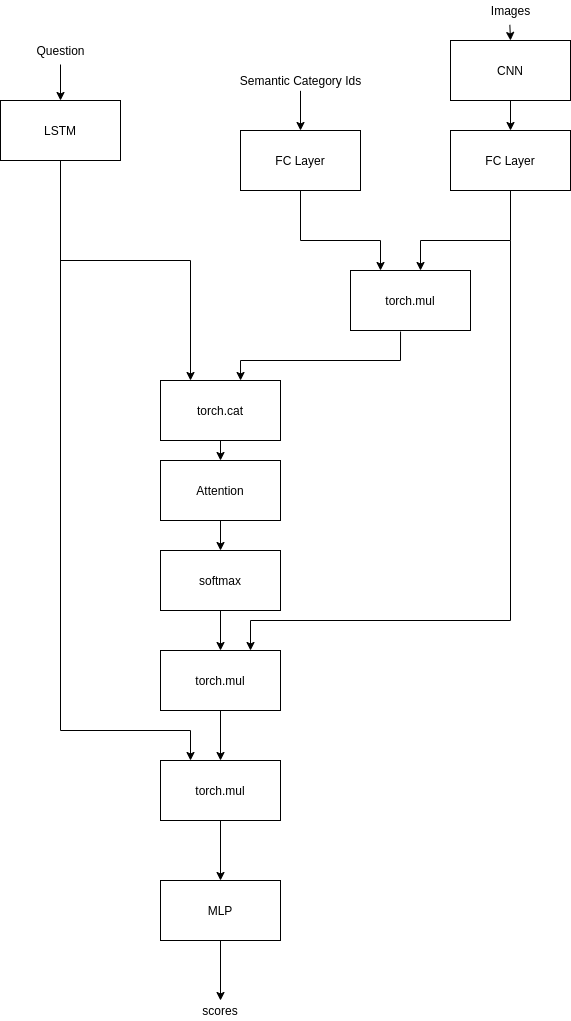
\includegraphics[width=.5\textwidth]{/home/yasmeen/Desktop/thesisproj/thesis/figure/model_w_semantic.png}
     \caption{Model With Semantic Category IDs as 3rd input}
     \label{fig:category_model}
\end{figure}


% RESULTS
% CREATED BY DAVID FRISK, 2016
\chapter{Results}
\section{Experiment 1: Baseline Evaluation \& Blindfolding}
Fig.~\ref{fig:training_metrics} shows metrics for each batch during training. Fig.~\ref{fig:baseline_metrics} shows metrics averaged for each epoch during the baseline evaluation. Fig.~\ref{fig:blindfolded_metrics} shows metrics averaged for each epoch during blindfolded evaluation. It's clear in this graphs that the evaluation results are more stable when the model is given images. As can be seen in Figures~\ref{fig:baseline_loss} \& ~\ref{fig:blindfolded_loss}, the model begins to overfit to the training data around epoch 10. 
Table~\ref{tab:best_baseline} shows the checkpoints with lowest loss, highest accuracy, and lowest mean rank during the evaluation of the baseline, with the metric that was "best" during that checkpoint in bold. Table~\ref{tab:best_blindfolded} shows the same for blindfolded evaluation. Comparing their best, the blindfolded model has 4.7\% worse loss than the baseline, 0.212 higher loss, and 0.149 higher mean rank. 

\begin{figure}
     \centering
     \begin{subfigure}[b]{0.3\textwidth}
         \centering
         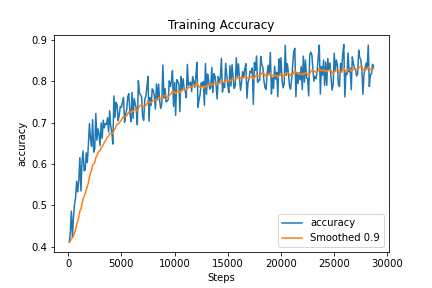
\includegraphics[width=\textwidth]{/home/yasmeen/Desktop/thesisproj/thesis/figure/results/baseline_and_blindfolding/training/accuracy.png}
         \caption{Training Accuracy}
         \label{fig:training_accuracy}
     \end{subfigure}
     \hfill
     \begin{subfigure}[b]{0.3\textwidth}
         \centering
         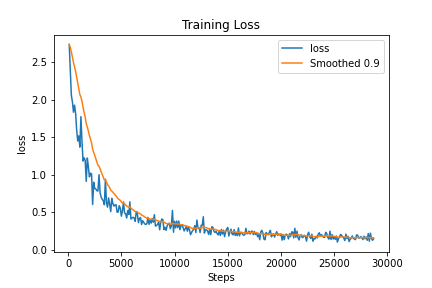
\includegraphics[width=\textwidth]{/home/yasmeen/Desktop/thesisproj/thesis/figure/results/baseline_and_blindfolding/training/loss.png}
         \caption{Training Loss}
         \label{fig:training_loss}
     \end{subfigure}
     \hfill
     \begin{subfigure}[b]{0.3\textwidth}
         \centering
         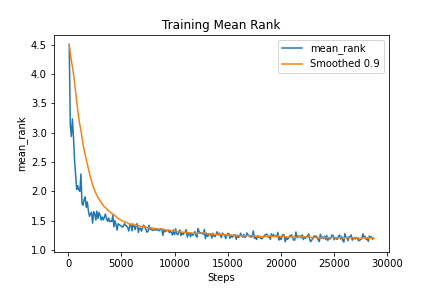
\includegraphics[width=\textwidth]{/home/yasmeen/Desktop/thesisproj/thesis/figure/results/baseline_and_blindfolding/training/mean_rank.png}
         \caption{Training Mean Rank}
         \label{fig:training_mean_rank}
     \end{subfigure}
     \caption{Training Metrics}
     \label{fig:training_metrics}
\end{figure}

\begin{figure}
     \centering
     \begin{subfigure}[b]{0.3\textwidth}
         \centering
         \includegraphics[width=\textwidth]{/home/yasmeen/Desktop/thesisproj/thesis/figure/results/baseline_and_blindfolding/images/avg val accuracy.png}
         \caption{Baseline Validation Accuracy}
         \label{fig:baseline_accuracy}
     \end{subfigure}
     \hfill
     \begin{subfigure}[b]{0.3\textwidth}
         \centering
         \includegraphics[width=\textwidth]{/home/yasmeen/Desktop/thesisproj/thesis/figure/results/baseline_and_blindfolding/images/avg val loss.png}
         \caption{Baseline Validation Loss}
         \label{fig:baseline_loss}
     \end{subfigure}
     \hfill
     \begin{subfigure}[b]{0.3\textwidth}
         \centering
         \includegraphics[width=\textwidth]{/home/yasmeen/Desktop/thesisproj/thesis/figure/results/baseline_and_blindfolding/images/avg val mean rank.png}
         \caption{Baseline Validation Mean Rank}
         \label{fig:baseline_mean_rank}
     \end{subfigure}
     \caption{Baseline Validation Metrics}
     \label{fig:baseline_metrics}
\end{figure}


\begin{figure}
     \centering
     \begin{subfigure}[b]{0.3\textwidth}
         \centering
         \includegraphics[width=\textwidth]{/home/yasmeen/Desktop/thesisproj/thesis/figure/results/baseline_and_blindfolding/blindfolded/avg val accuracy.png}
         \caption{Blindfolded Validation Accuracy}
         \label{fig:blindfolded_accuracy}
     \end{subfigure}
     \hfill
     \begin{subfigure}[b]{0.3\textwidth}
         \centering
         \includegraphics[width=\textwidth]{/home/yasmeen/Desktop/thesisproj/thesis/figure/results/baseline_and_blindfolding/blindfolded/avg val loss.png}
         \caption{Blindfolded Validation Loss}
         \label{fig:blindfolded_loss}
     \end{subfigure}
     \hfill
     \begin{subfigure}[b]{0.3\textwidth}
         \centering
         \includegraphics[width=\textwidth]{/home/yasmeen/Desktop/thesisproj/thesis/figure/results/baseline_and_blindfolding/blindfolded/avg val mean rank.png}
         \caption{Blindfolded Validation Mean Rank}
         \label{fig:blindfolded_mean_rank}
     \end{subfigure}
     \caption{Blindfolded Validation Metrics}
     \label{fig:blindfolded_metrics}
\end{figure}

\begin{table}[h]
\centering
\caption{"Best" Epochs During Baseline Evaluation}
\begin{tabular}{l | l | l | l}
Checkpoint & Loss & Accuracy & Mean Rank \\
\hline
8 & \textbf{2.204141} & 0.381122 & 4.341837 \\
15 & 2.404433 & \textbf{0.403061} & 4.138265 \\
23 & 2.691763 & 0.370408 & \textbf{4.110714}
\end{tabular}
\label{tab:best_baseline}
\end{table}

\begin{table}[h]
\centering
\caption{"Best" Epochs During Blindfolded Evaluation}
\begin{tabular}{l | l | l | l}
Checkpoint & Loss & Accuracy & Mean Rank \\
\hline
5 & \textbf{2.416477} & 0.246429 & 5.493877 \\
27 & 2.546098 & \textbf{0.355612} & 4.551021 \\
39 & 4.788071 & 0.307653 & \textbf{4.260204}
\end{tabular}
\label{tab:best_blindfolded}
\end{table}




% CONCLUSION
% CREATED BY DAVID FRISK, 2016
\chapter{Conclusion}

You may consider to instead divide this chapter into discussion of the results and a summary. 

\section{Discussion}

\section{Conclusion}


% REFERENCES / BIBLIOGRAPHY
\cleardoublepage
\addcontentsline{toc}{chapter}{Bibliography}
% CREATED BY DAVID FRISK, 2016
\bibliography{references}


% APPENDICES
\cleardoublepage
\appendix
\setcounter{page}{1}
\pagenumbering{Roman}			% Capitalized roman numbering starting from I (one)

\begin{appendices}
\chapter{Matterport3D Semantic Categories}
\begin{table}[h!]
\label{app:categories}
\centering
\begin{adjustbox}{totalheight=.65\textheight}
\begin{tabular}{|l|l|}
\hline
id & category \\
\hline
	0 & void \\
	1 & wall \\
	2 & floor \\
	3 & chair \\
	4 & door \\
	5 & table \\
	6 & picture \\
	7 & cabinet \\
	8 & cushion \\
	9 & window \\
	10 & sofa \\
	11 & bed \\
	12 & curtain \\
	13 & chest of drawers \\
	14 & plant \\
	15 & sink \\
	16 & stairs \\
	17 & ceiling \\
	18 & toilet \\
	19 & stool \\
	20 & towel \\
	21 & mirror \\
	22 & TV monitor \\
	23 & shower \\
	24 & column \\
	25 & bathtub \\
	26 & counter \\
	27 & fireplace \\
	28 & lighting \\
	29 & beam \\
	30 & railing \\
	31 & shelving \\
	32 & blinds \\
	33 & gym equipment \\
	34 & seating \\
	35 & board panel \\
	36 & furniture \\
	37 & appliances \\
	38 & clothes \\
	39 & objects \\
	40 & misc \\
	41 & unlabelled \\
	\hline
\end{tabular}
\end{adjustbox}
\end{table}
\end{appendices}



\end{document}